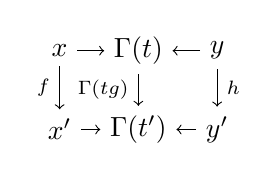
\begin{tikzpicture}
\node (v1) at (0,1) {$x$};
\node (v2) at (1,1) {$\Gamma (t)$};
\node (v3) at (2,1) {$y$};
\node (v4) at (0,0) {$x'$};
\node (v5) at (1,0) {$\Gamma (t')$};
\node (v6) at (2,0) {$y'$};
\draw [->] (v1) edge (v2);
\draw [->] (v3) edge (v2);
\draw [->] (v4) edge (v5);
\draw [->] (v6) edge (v5);
\draw [->] (v1) edge node [left] {\scriptsize $f$} (v4);
\draw [->] (v2) edge node [left] {\scriptsize $\Gamma (tg)$} (v5);
\draw [->] (v3) edge node [right] {\scriptsize $h$} (v6);
\end{tikzpicture}